
\section{Bedienoberfläche}

Hier sollen die Skizzen/Prototypen von Bedienoberflächen dargestellt werden, als auch die Zusammenhänge zwischen denen (wie gelingt man von einem zu dem anderen Fenster/Ansicht). Ein Beispiel für Bildereinbau in LaTeX ist die Abbildung~\ref{gui:zusammenhang}.\footnote{Bevor Sie mit den Skizzen anfangen, überlegen Sie sich, welche virtuelle Räume im System zu haben sind und dann halte Sie die Namen der GUI-Fenstern mit diesen konsistent.}

\newcounter{gui}\setcounter{gui}{10}

\begin{description}[leftmargin=5em, style=sameline]	
	\begin{lhp}{gui}{GUI}{gui:vorraum}
		\item[Name:] Vorraum-Interface
		\item[Beschreibung:] Interface für Anmeldung
		\item[Relevante Systemfunktionen:] \ref{funk:zugriff}
		\item[Abbildungen:] \ref{gui:vorraum}
	\end{lhp}
\end{description}


\begin{description}[leftmargin=5em, style=sameline]	
	\begin{lhp}{gui}{GUI}{gui:registrierung}
		\item[Name:] Registrierung-Interface
		\item[Beschreibung:] Interface für Registrierung
		\item[Relevante Systemfunktionen:] \ref{funk:zugriff}
		\item[Abbildungen:]  \ref{gui:register}
	\end{lhp}
\end{description}

\begin{comment}
\begin{description}[leftmargin=5em, style=sameline]	
	\begin{lhp}{gui}{GUI}{gui:beispiel}
		\item[Name:] Änderung des Passworts
		\item[Beschreibung:] Änderung des Passworts ,wenn es verloren geht oder nach dem Will des Spielers.
		\item[Relevante Systemfunktionen:] /LF20/
		\item[Abbildungen:] \ref{gui:Passworts}
	\end{lhp}
\end{description}
\end{comment} % Das muss weg oder


\begin{description}[leftmargin=5em, style=sameline]	
	\begin{lhp}{gui}{GUI}{gui:lobby}
		\item[Name:] Lobby 
		\item[Beschreibung:] Lobby in der sich alle angemeldeten Spieler versammeln können. Von dort aus kann man Spielräume erstellen, das Regelwerk betrachten, Spielräumen beitreten, die aktuell angemeldeten Benutzer sehen, chatten, sich abmelden und seinen Account löschen.  
		\item[Relevante Systemfunktionen:] \ref{funk:spielraum}
		\item[Abbildungen:] \ref{gui:lobby}
	\end{lhp}
\end{description}



\begin{description}[leftmargin=5em, style=sameline]	
	\begin{lhp}{gui}{GUI}{gui:bestenliste}
		\item[Name:] Bestenliste
		\item[Beschreibung:] Zeigt welche Spieler im aktuellen Raum am meisten Spiele gewonnen haben und erstellt.  
		\item[Relevante Systemfunktionen:] \ref{funk:bestenliste}
		\item[Abbildungen:] \ref{gui:bestenliste}
	\end{lhp}
\end{description}

\begin{description}[leftmargin=5em, style=sameline]	
	\begin{lhp}{gui}{GUI}{gui:srerstellen}
		\item[Name:] Spielraum erstellen
		\item[Beschreibung:]  Fenster für die Erstellung eines Spielraums. Es können der Raumname, so wie die Spieleranzahl für den festgelegt werden.
		\item[Relevante Systemfunktionen:] \ref{funk:spielraum}
		\item[Abbildungen:] \ref{gui:erstellen}
	\end{lhp}
\end{description}

\begin{description}[leftmargin=5em, style=sameline]	
	\begin{lhp}{gui}{GUI}{gui:srlöschen}
		\item[Name:] Spielraum löschen
		\item[Beschreibung:]  Fenster für die Löschung des Spielraums.
		\item[Relevante Systemfunktionen:] \ref{funk:spielraum}
		\item[Abbildungen:] \ref{gui:srlöschen}
	\end{lhp}
\end{description}


\begin{description}[leftmargin=5em, style=sameline]	
	\begin{lhp}{gui}{GUI}{gui:srändern}
		\item[Name:] Spielraum ändern
		\item[Beschreibung:] Fenster für die Änderung des Raumnamens, der Anzahl an Spielern.
		\item[Relevante Systemfunktionen:] \ref{funk:spielraum}
		\item[Abbildungen:] \ref{gui:srändern}
	\end{lhp}
\end{description}



\begin{description}[leftmargin=5em, style=sameline]	
	\begin{lhp}{gui}{GUI}{gui:logout}
		\item[Name:] Spieler abmelden
		\item[Beschreibung:]  Fenster, in dem sich der Spieler aus dem System abmeldet.
		\item[Relevante Systemfunktionen:] \ref{funk:zugriff}
		\item[Abbildungen:] \ref{gui:abmelden}
	\end{lhp}
\end{description}



\begin{description}[leftmargin=5em, style=sameline]	
	\begin{lhp}{gui}{GUI}{gui:slöschen}
		\item[Name:] Spieler löschen
		\item[Beschreibung:]  Fenster, in dem der Spieler sein Konto löschen kann.
		\item[Relevante Systemfunktionen:] \ref{funk:zugriff}
		\item[Abbildungen:] \ref{gui:splöschen}
	\end{lhp}
\end{description}


\begin{comment}

\begin{description}[leftmargin=5em, style=sameline]	
	\begin{lhp}{gui}{GUI}{gui:spielraum}
		\item[Name:] Spielraum
		\item[Beschreibung:] Fenster, in dem die Einstellungen des Spiels festgelegt, der Raum verlassen und das Spiel gestartet werden kann. Nachdem das Spiel gestartet wurde wird hier das eigentliche Spiel gespielt. Gleichzeitig gibt es noch einen Chat, damit sich die Spieler austauschen können.
		\item[Relevante Systemfunktionen:] \ref{funk:spielverw}
		\item[Abbildungen:] \ref{gui:spielraum}
	\end{lhp}
\end{description}

\end{comment}

\begin{description}[leftmargin=5em, style=sameline]	
	\begin{lhp}{gui}{GUI}{gui:spielraum_h}
		\item[Name:] Spielraum Fenster eines Hosts
		\item[Beschreibung:] Fenster, in dem der Host vor dem Starten des Spiels die Einstellungen des Spiels ändern, den Raum verlassen, Bots hinzufügen und das Spiel starten kann. Nachdem das Spiel über den entsprechenden Knopf gestartet wurde, wird hier das eigentliche Spiel gespielt. Die Knöpfe zum Hinzufügen eines Bots, zum Ändern, Verlassen oder Löschen des Raumes und zum Starten des Spiels können dann nicht mehr betätigt werden. Weiterhin gibt es noch einen Chat, damit sich die Spieler austauschen können und eine Raum-lokale Bestenliste, sodass man sehen kann, welcher Spieler im Raum bisher wie viele Spiele gewonnen hat.
		\item[Relevante Systemfunktionen:] \ref{funk:spielverw}
		\item[Abbildungen:] \ref{gui:spielraumnichtvoll_h}, \ref{gui:spielraumstarten_h}, \ref{gui:spielraumgestartet_h}
	\end{lhp}
\end{description}


\begin{description}[leftmargin=5em, style=sameline]	
	\begin{lhp}{gui}{GUI}{gui:spielraum_s}
		\item[Name:] Spielraum Fenster eines beigetretenen Spielers
		\item[Beschreibung:] Fenster, in dem der beigetretene Spieler vor dem Starten des Spiels wartet. Nachdem das Spiel vom Host des Raumes gestartet wurde, wird hier das eigentliche Spiel gespielt. Der Raum verlassen Knopf kann daraufhin nicht mehr betätigt werden. Weiterhin gibt es noch einen Chat, damit sich die Spieler austauschen können und eine Raum-lokale Bestenliste, sodass man sehen kann, welcher Spieler im Raum bisher wie viele Spiele gewonnen hat.
		\item[Relevante Systemfunktionen:] \ref{funk:spielverw}
		\item[Abbildungen:] \ref{gui:spielraumnichtvoll_s}, \ref{gui:spielraumstarten_s}, \ref{gui:spielraumgestartet_s}
	\end{lhp}
\end{description}


\begin{description}[leftmargin=5em, style=sameline]	
	\begin{lhp}{gui}{GUI}{gui:spielverlassen}
		\item[Name:] Spiel verlassen
		\item[Beschreibung:] Fenster, mit dem man das Spiel verlassen kann. 
		\item[Relevante Systemfunktionen:] \ref{funk:spielverw}
		\item[Abbildungen:] \ref{gui:verlassen}
	\end{lhp}
\end{description}

\begin{description}[leftmargin=5em, style=sameline]	
	\begin{lhp}{gui}{GUI}{gui:regelwerk}
		\item[Name:] Regelwerk
		\item[Beschreibung:] Fenster, in dem die Regeln des Spiels erklärt werden.
		\item[Relevante Systemfunktionen:] \ref{funk:regel}\\
		\item[Abbildungen:] \ref{gui:spielregeln}
	\end{lhp}
\end{description}

\begin{description}[leftmargin=5em, style=sameline]	
	\begin{lhp}{gui}{GUI}{gui:spielbeendet}
		\item[Name:] Spiel beendet
		\item[Beschreibung:] Fenster, das den Sieger des Spiels anzeigt.
		\item[Relevante Systemfunktionen:] \ref{funk:spielverw}
		\item[Abbildungen:] \ref{gui:gewonnen}
	\end{lhp}
\end{description}


\begin{description}[leftmargin=5em, style=sameline]	
	\begin{lhp}{gui}{GUI}{gui:beispiel}
		\item[Name:] Zusammenhänge
		\item[Beschreibung:] Zusammenhänge zwischen GUI-Ansichten
		\item[Relevante Systemfunktionen:] Alle
		\item[Abbildungen:] \ref{gui:zusammenhang}
	\end{lhp}
\end{description}

\break


\begin{figure}[h]
	\centering
	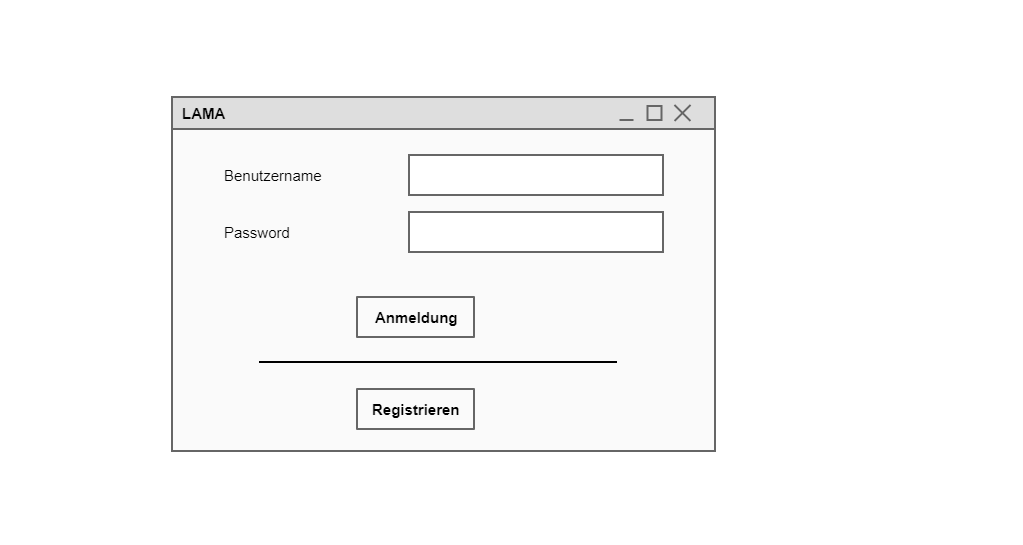
\includegraphics[width=\textwidth]{img/Vorraum.png}
	\caption{Darstellung des Vorrauminterface.}
	\label{gui:vorraum}
\end{figure}

\begin{figure}[h]
	\centering
	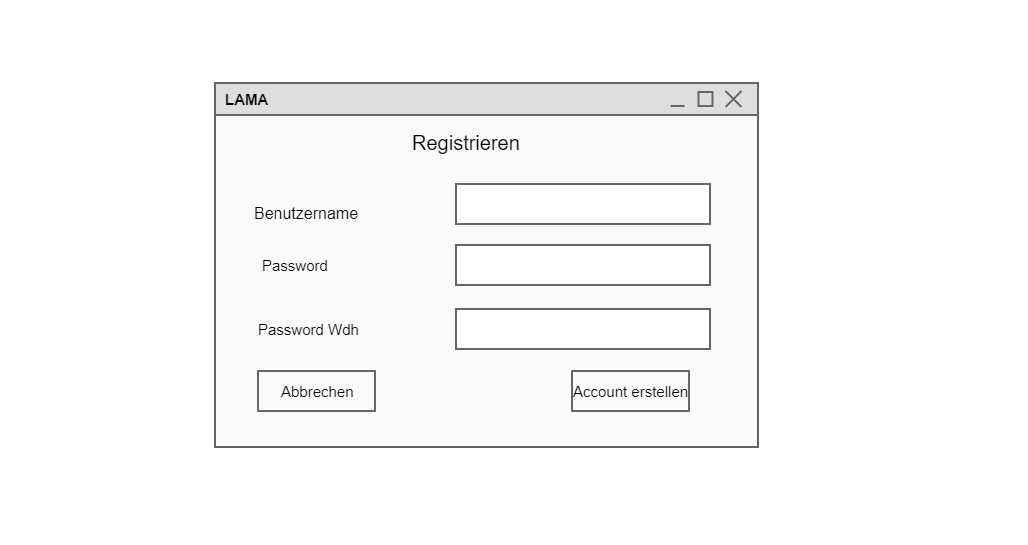
\includegraphics[width=\textwidth]{img/registrierungsinterface.png}
	\caption{Darstellung des Registrierungsinterface.}
	\label{gui:register}
\end{figure}

\begin{figure}[h]
	\centering
	\includegraphics[width=\textwidth]{img/spielregeln.png}
	\caption{Darstellung des Spielregeln Interface.}
	\label{gui:spielregeln} %ändern
\end{figure}

\begin{figure}[h]
	\centering
	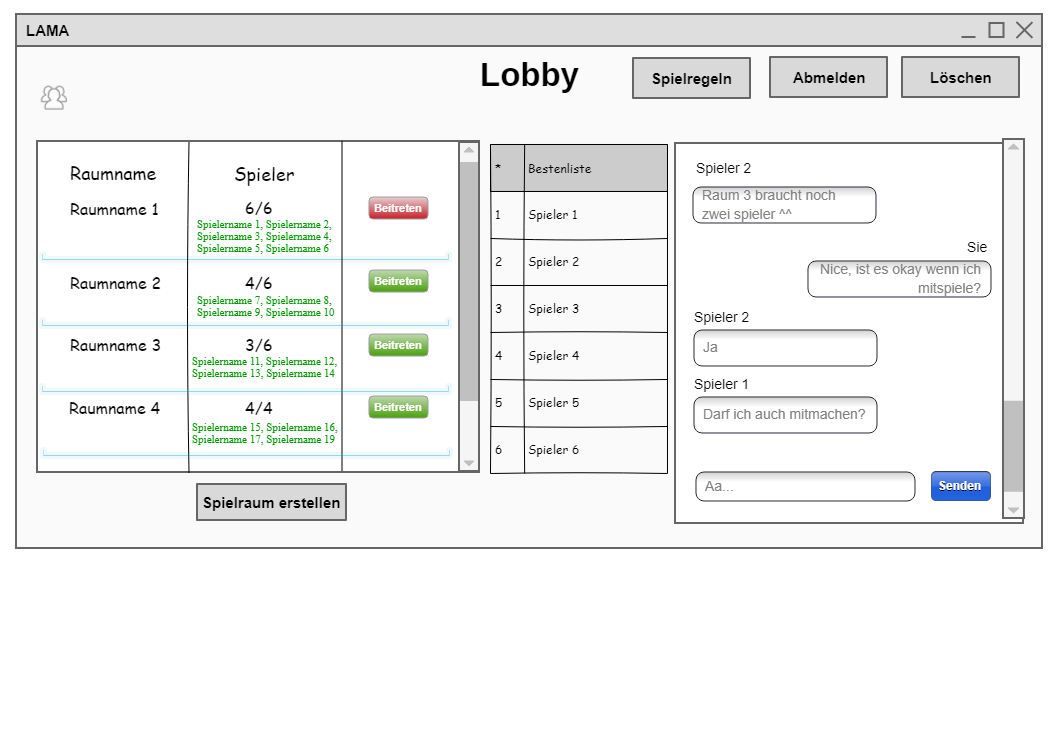
\includegraphics[width=\textwidth]{img/lobby.png}
	\caption{Darstellung des Lobbysinterface.}
	\label{gui:lobby} %ändern
\end{figure}

\begin{figure}[h]
	\centering
	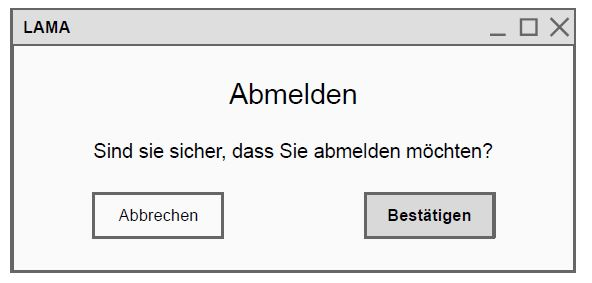
\includegraphics[width=\textwidth]{img/spielerabmelden.JPG}
	\caption{Darstellung des Abmeldensinterface.}
	\label{gui:abmelden} %ändern
\end{figure}

\begin{figure}[h]
	\centering
	\includegraphics[width=\textwidth]{img/spielerlöschen.JPG}
	\caption{Darstellung des Spieler löschen Interface.}
	\label{gui:splöschen} %ändern
\end{figure}

\begin{figure}[h]
	\centering
	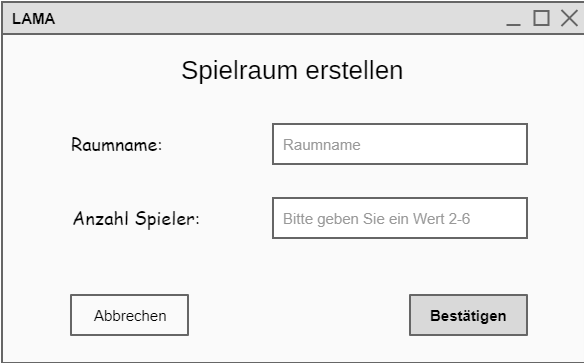
\includegraphics[width=\textwidth]{img/srerstellen.png}
	\caption{Darstellung des Spielraum erstellen Interface.}
	\label{gui:erstellen} %ändern
\end{figure}

\begin{figure}[h]
	\centering
	\includegraphics[width=\textwidth]{img/spielraumnichtvoll.png}
	\caption{Spielraumsinterface des Spielraum-Hosts. Der Spielraum ist noch nicht voll.}
	\label{gui:spielraumnichtvoll_h} 
\end{figure}

\begin{figure}[h]
	\centering
	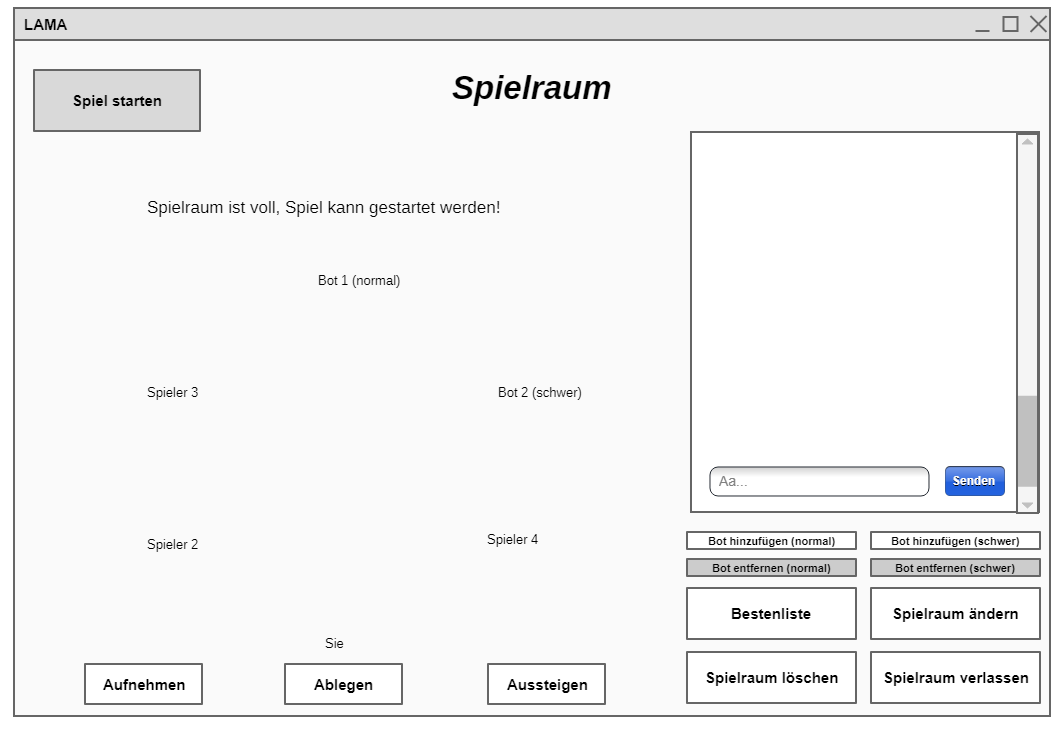
\includegraphics[width=\textwidth]{img/Spielstarten.png}
	\caption{Spielraumsinterface des Spielraum-Hosts. Der Spielraum ist voll und kann gestartet werden.}
	\label{gui:spielraumstarten_h} 
\end{figure}

\begin{figure}[h]
	\centering
	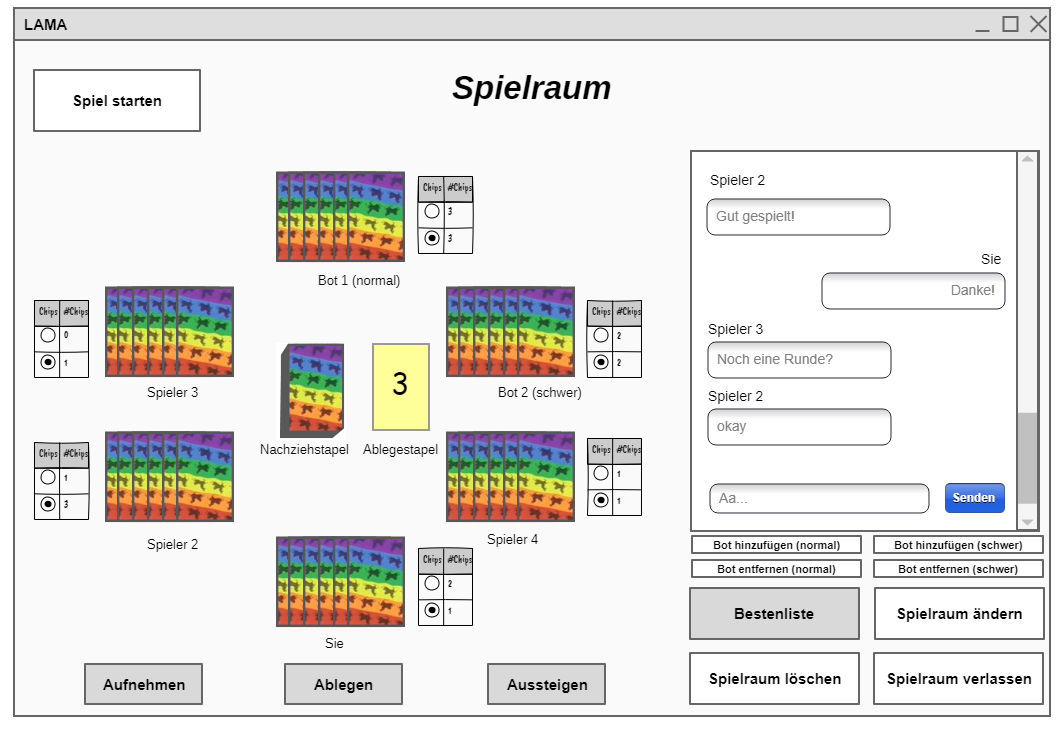
\includegraphics[width=\textwidth]{img/spielgestartet.png}
	\caption{Spielraumsinterface des Spielraum-Hosts. Das Spiel wurde gestartet.}
	\label{gui:spielraumgestartet_h} 
\end{figure}

\begin{figure}[h]
	\centering
	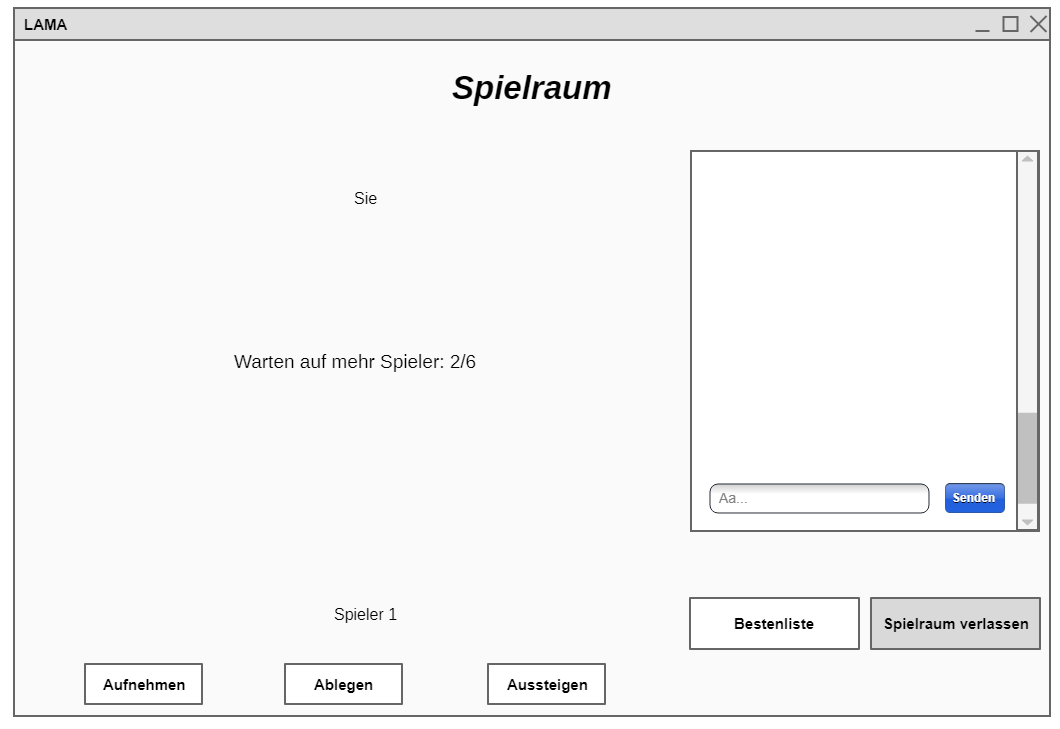
\includegraphics[width=\textwidth]{img/spielraumnichtvollbeigetretenerspielerv2.png}
	\caption{Spielraumsinterface eines in den Raum beigetretenen Spielers. Der Spielraum ist noch nicht voll.}
	\label{gui:spielraumnichtvoll_s} 
\end{figure}

\begin{figure}[h]
	\centering
	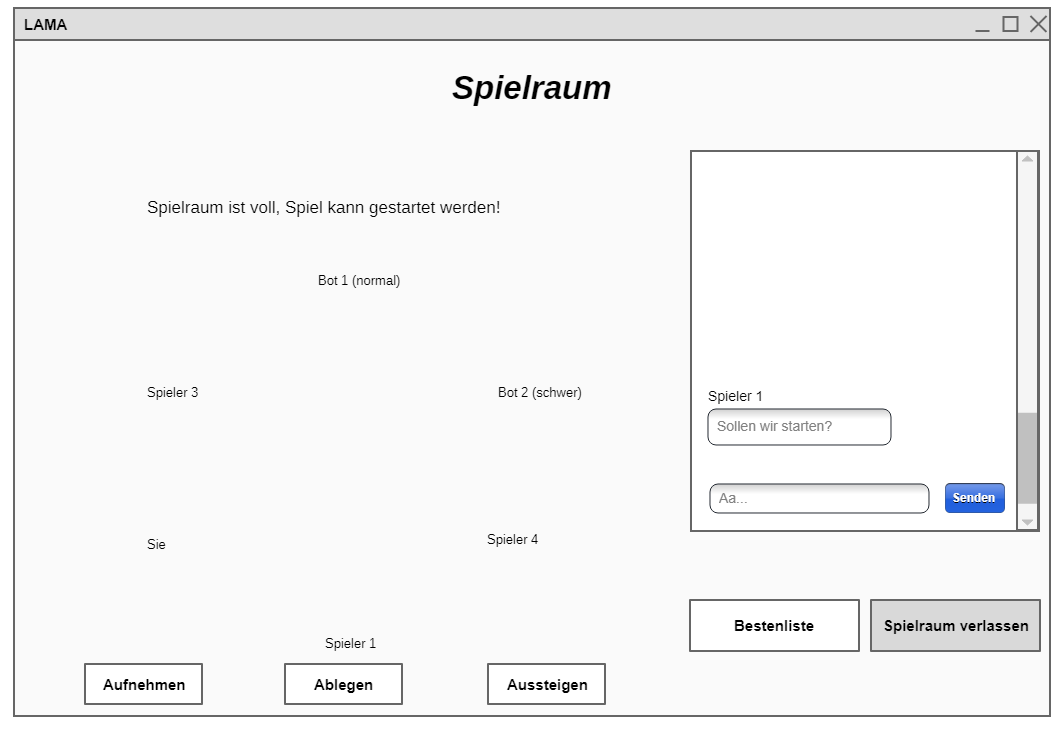
\includegraphics[width=\textwidth]{img/spielstartenbeigetretenerspielerv3.png}
	\caption{Spielraumsinterface eines in den Raum beigetretenen Spielers. Der Spielraum ist voll und kann gestartet vom Host werden.}
	\label{gui:spielraumstarten_s} 
\end{figure}

\begin{figure}[h]
	\centering
	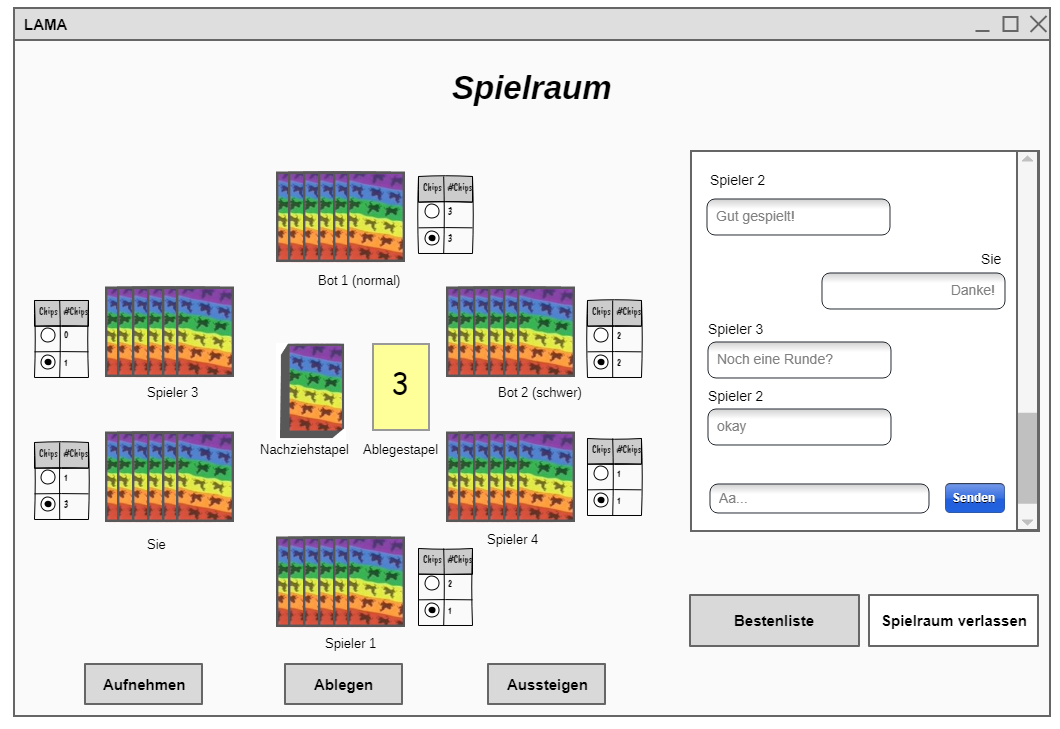
\includegraphics[width=\textwidth]{img/spielgestartetbeigetretenerspielerv3.png}
	\caption{Spielraumsinterface eines in den Raum beigetretenen Spielers. Das Spiel wurde gestartet.}
	\label{gui:spielraumgestartet_s} 
\end{figure}

\begin{figure}[h]
	\centering
	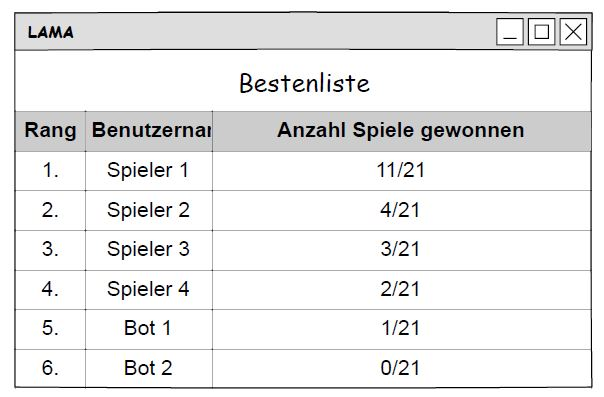
\includegraphics[width=\textwidth]{img/Bestenliste.JPG}
	\caption{Darstellung des Bestenliste Interface.}
	\label{gui:bestenliste} %ändern
\end{figure}

\begin{figure}[h]
	\centering
	\includegraphics[width=\textwidth]{img/srändern.png}
	\caption{Darstellung des Spielraum ändern Interface.}
	\label{gui:srändern} %ändern
\end{figure}

\begin{figure}[h]
	\centering
	\includegraphics[width=\textwidth]{img/srlöschen.png}
	\caption{Darstellung des Spielraum löschen Interface.}
	\label{gui:srlöschen} %ändern
\end{figure}

\begin{figure}[h]
	\centering
	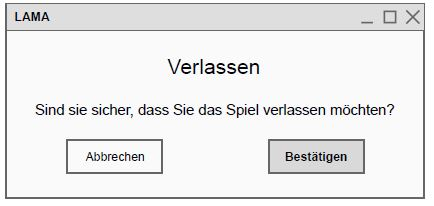
\includegraphics[width=\textwidth]{img/verlassen.JPG}
	\caption{Darstellung des Spielraum verlassen Interface.}
	\label{gui:verlassen} %ändern
\end{figure}

\begin{figure}[h]
	\centering
	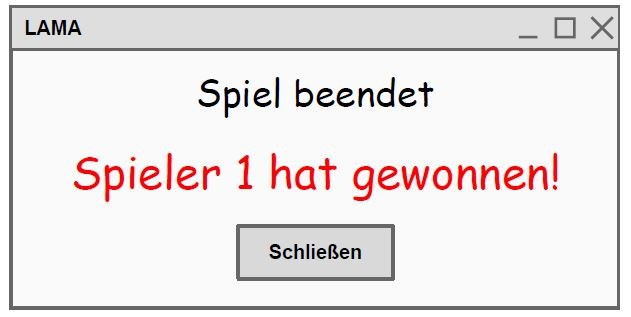
\includegraphics[width=\textwidth]{img/gewonnen.JPG}
	\caption{Darstellung des Spieler X hat gewonnen Interface.}
	\label{gui:gewonnen} %ändern
\end{figure}

\begin{figure}[h]
	\centering
	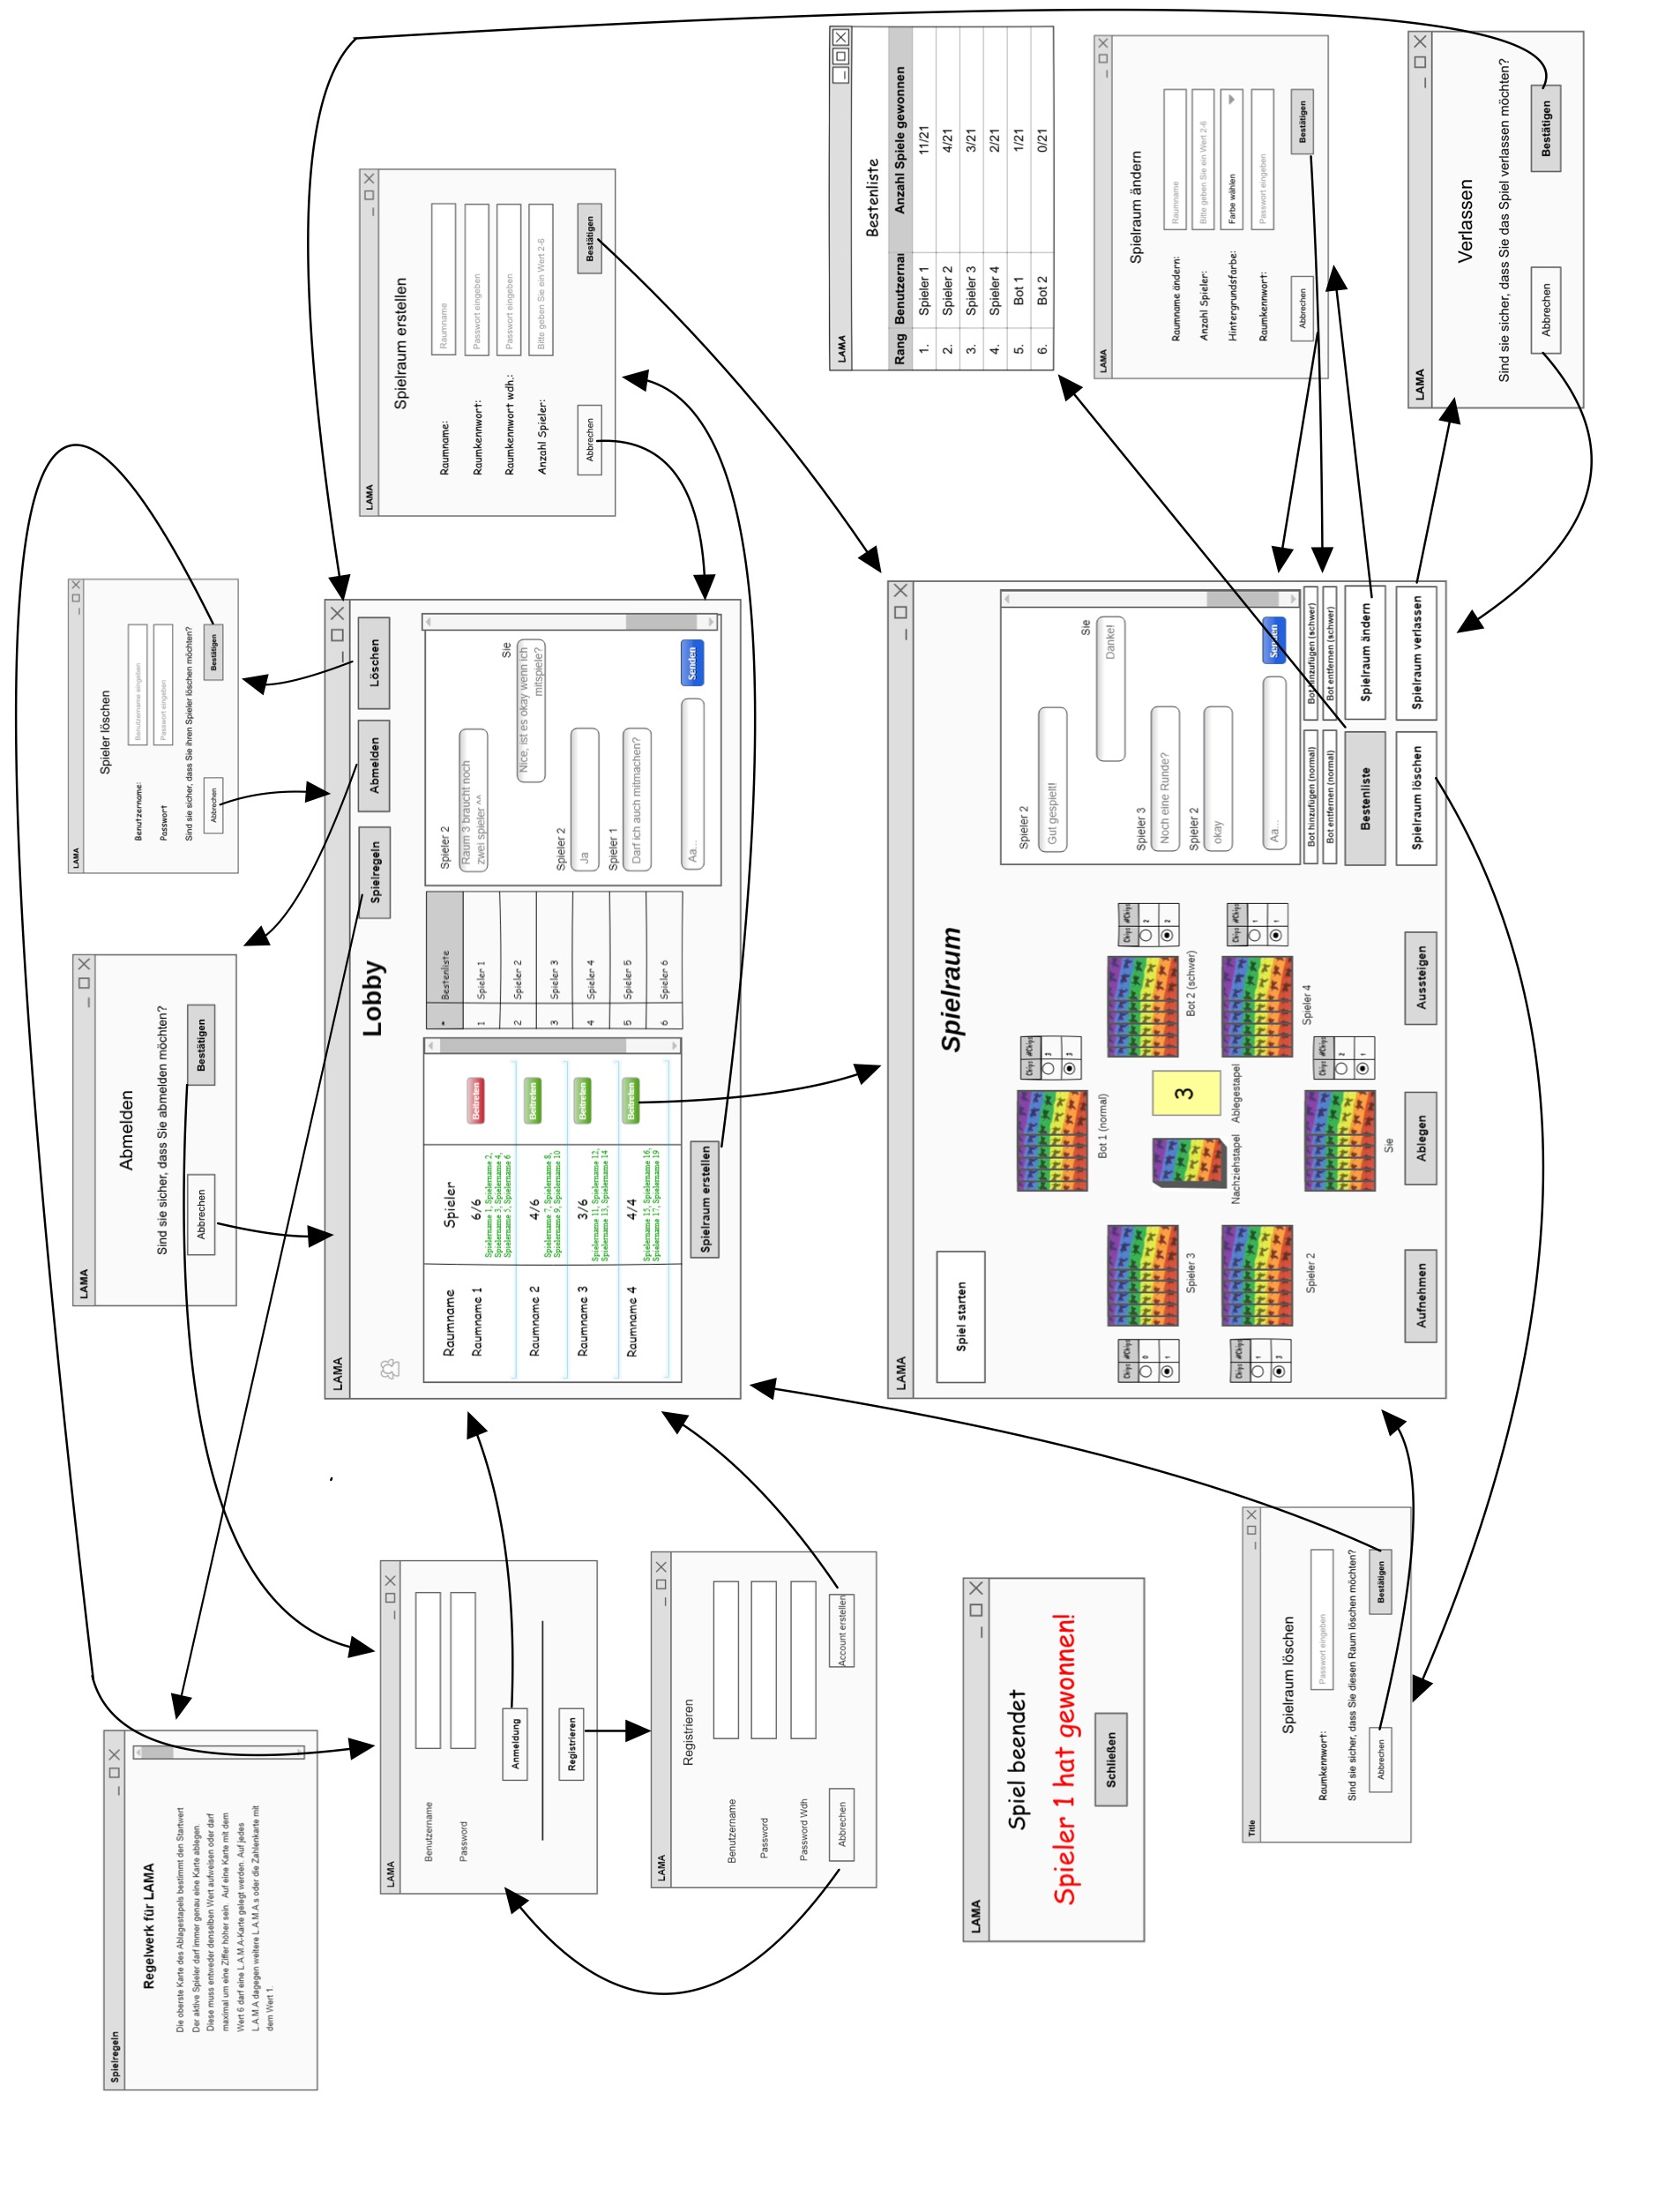
\includegraphics[width=0.9\textwidth,height=0.6\textwidth]{img/gui-zusammenhang.jpg}
	\caption{Darstellung der Zusammenhänge zwischen GUI-Ansichten .}
	\label{gui:zusammenhang}
\end{figure}


